\section{Aufgabe E37}
\begin{figure}[!htbp]
\centering
\fbox{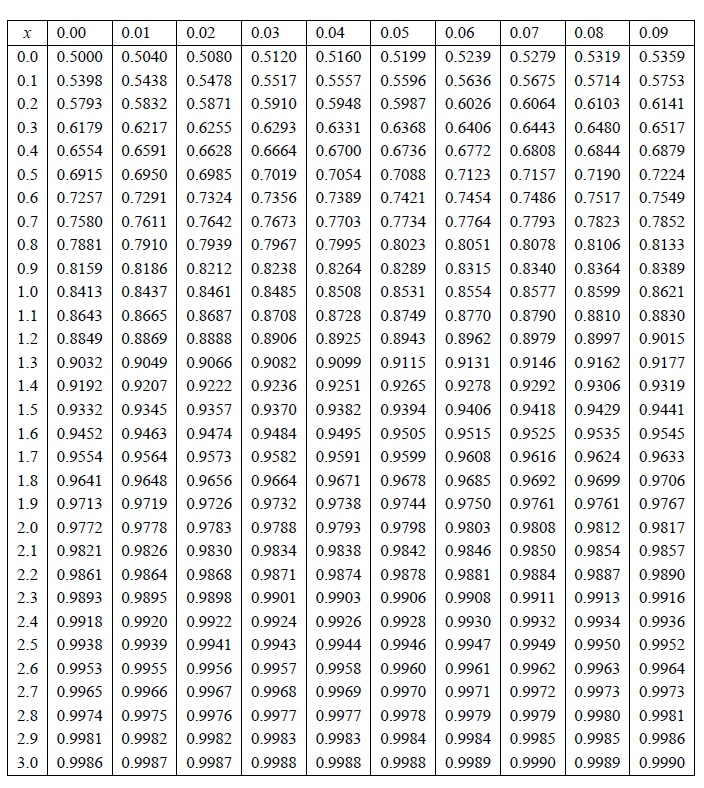
\includegraphics[width=0.9\linewidth]{./chapters/Grafiken_TB/TB_E37.jpg}}
\end{figure}
Die Laktationsleistung bei einem weiblichen Rind aus einer speziellen Population (Milchleistung zwischen zwei Geburten, gemessen in kg) lasse sich ausreichend genau durch eine N(4000, $10^6$) - verteilte Zufallsvariable beschreiben.
\begin{enumerate}[leftmargin=1cm, label=\alph*)]
\item Berechnen Sie die Wahrscheinlichkeit, dass eine zuf�llig aus der Population herausgegriffene Kuh eine Laktationsleistung von
\begin{enumerate}[leftmargin=1cm, label=\roman*)]
\item weniger als 3000 kg hat
\item mehr als 6000 kg hat.
\end{enumerate}
\item Welche Laktationsleistung muss eine Kuh mindestens erbringen, um nicht zu den schlechtesten 33\% dieser Population (in Bezug auf die Laktationsleistung) zu geh�ren?
\item Eine Herde aus Rindern dieser Population bestehe aus 100 K�hen. Welche Mittelwert und welche Varianz besitzt die Milchleistung dieser Herde, falls vorausgesetzt wird, dass die Laktationsleistungen der K�he stochastisch unabh�ngig ist?
\end{enumerate}
